\documentclass{standalone}
\usepackage{tikz}
\usetikzlibrary{patterns}
\usetikzlibrary{positioning}
\usetikzlibrary{patterns, positioning}
\usetikzlibrary{shapes.misc}
\usepackage[outline]{contour}
\contourlength{1.5pt} 
\usepackage[sfdefault]{ClearSans}

\begin{document}
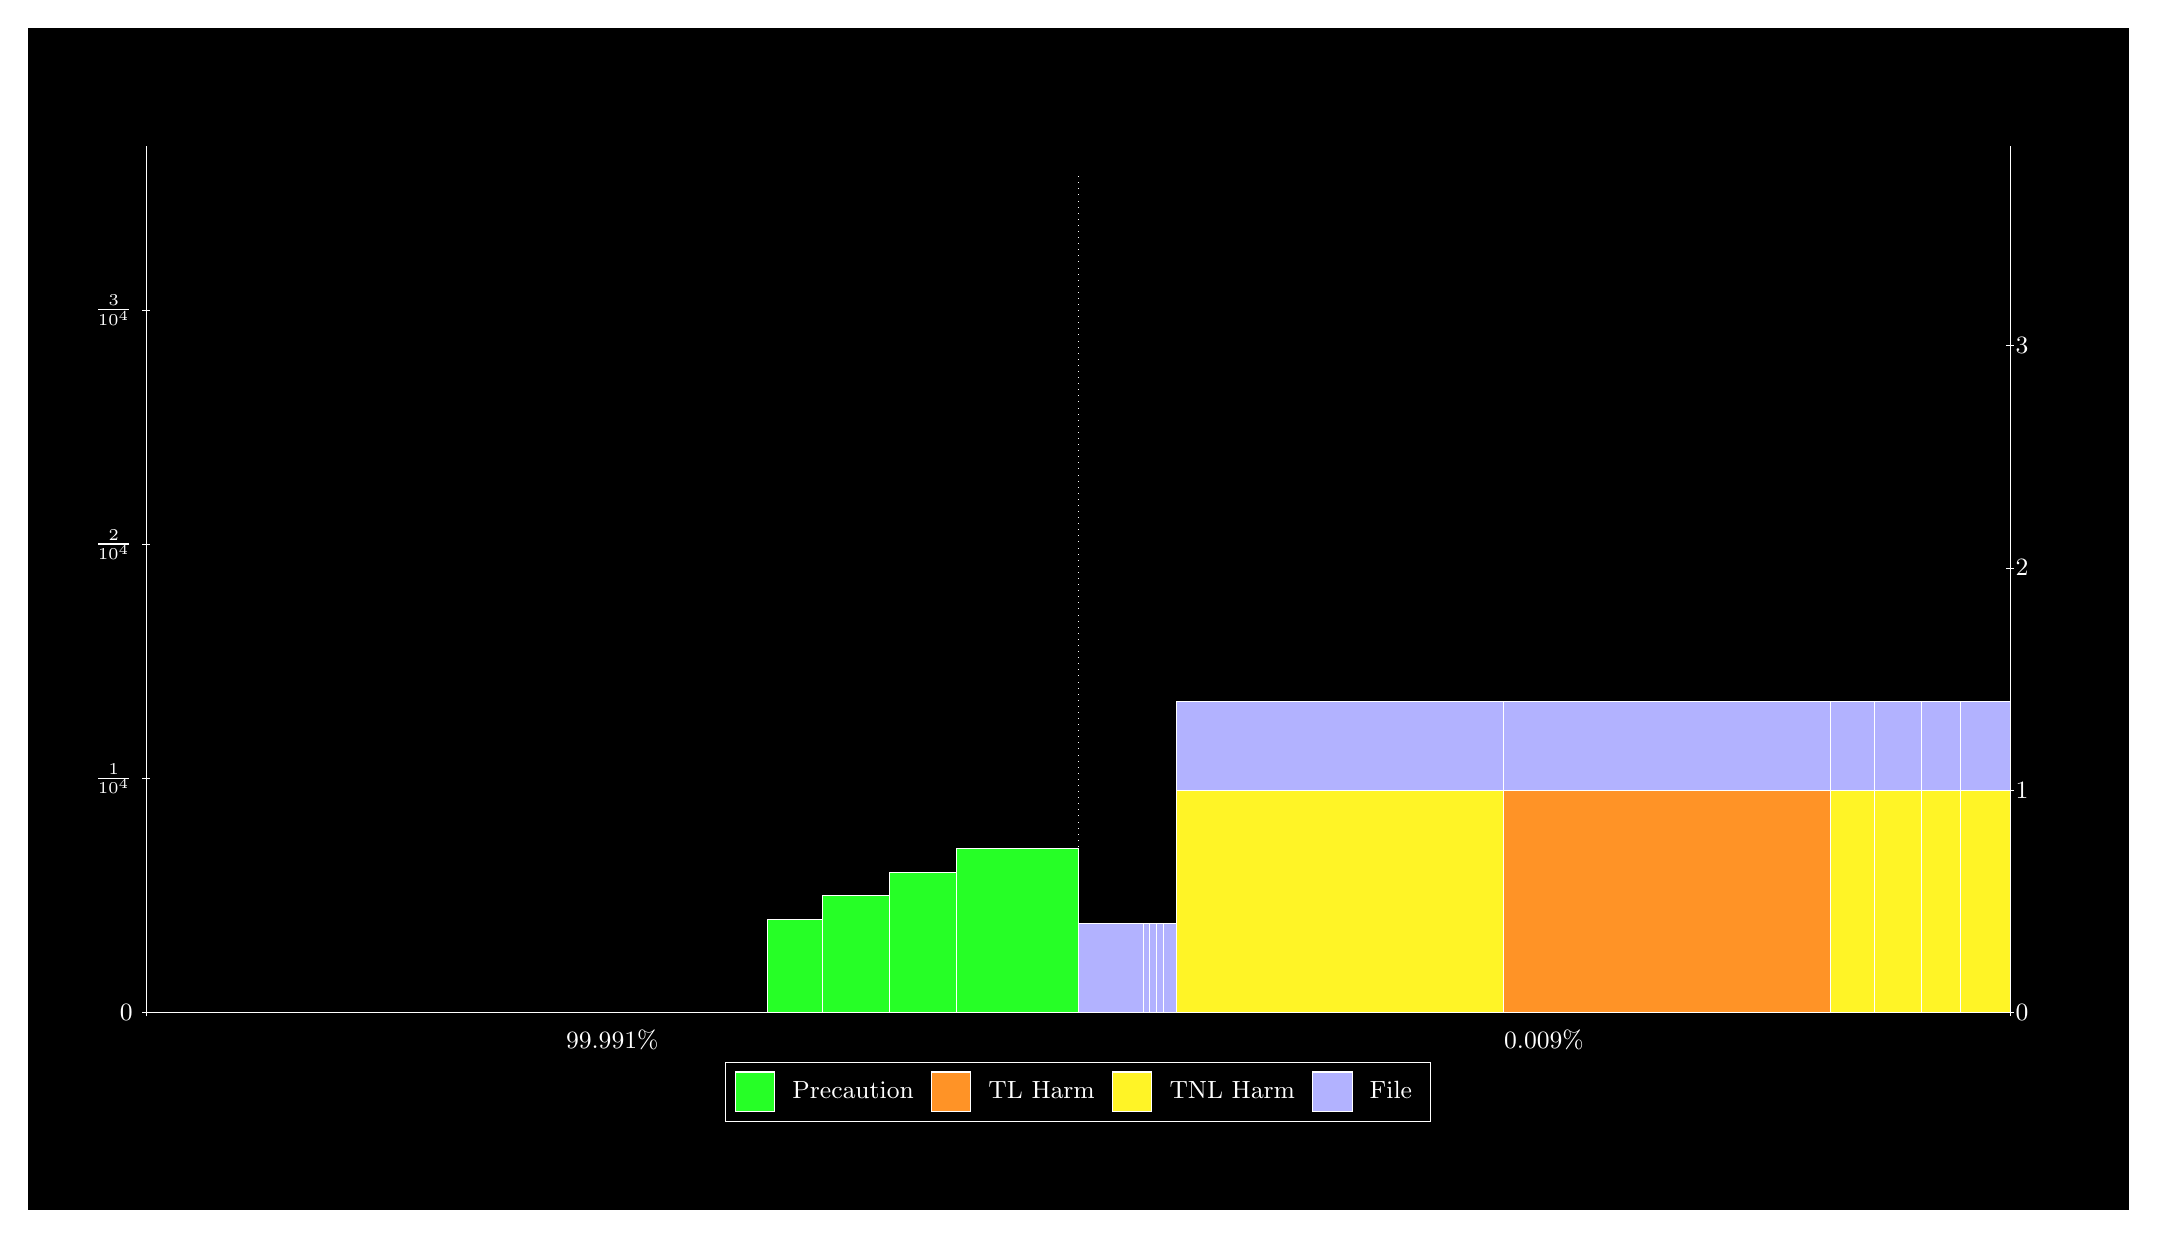
\begin{tikzpicture}
\draw[fill=black] (0,0) rectangle (26.667,15);
\draw[fill=green!85,draw=white,very thin] (9.3887,2.5) rectangle (10.088,3.6891);
\draw[fill=green!85,draw=white,very thin] (10.088,2.5) rectangle (10.936,3.9863);
\draw[fill=green!85,draw=white,very thin] (10.936,2.5) rectangle (11.786,4.2836);
\draw[fill=green!85,draw=white,very thin] (11.786,2.5) rectangle (13.333,4.5809);
\draw[fill=blue!30,draw=white,very thin] (13.333,2.5) rectangle (14.164,3.6293);
\draw[fill=green!85,draw=white,very thin] (14.164,2.5) rectangle (14.237,2.5001);
\draw[fill=blue!30,draw=white,very thin] (14.164,2.5001) rectangle (14.237,3.6294);
\draw[fill=green!85,draw=white,very thin] (14.237,2.5) rectangle (14.326,2.5001);
\draw[fill=blue!30,draw=white,very thin] (14.237,2.5001) rectangle (14.326,3.6294);
\draw[fill=green!85,draw=white,very thin] (14.326,2.5) rectangle (14.415,2.5002);
\draw[fill=blue!30,draw=white,very thin] (14.326,2.5002) rectangle (14.415,3.6295);
\draw[fill=green!85,draw=white,very thin] (14.415,2.5) rectangle (14.581,2.5002);
\draw[fill=blue!30,draw=white,very thin] (14.415,2.5002) rectangle (14.581,3.6295);
\draw[fill=yellow!85,draw=white,very thin] (14.581,2.5) rectangle (18.736,5.3232);
\draw[fill=blue!30,draw=white,very thin] (14.581,5.3232) rectangle (18.736,6.4525);
\draw[fill=orange!85,draw=white,very thin] (18.736,2.5) rectangle (22.888,5.3232);
\draw[fill=blue!30,draw=white,very thin] (18.736,5.3232) rectangle (22.888,6.4525);
\draw[fill=green!85,draw=white,very thin] (22.888,2.5) rectangle (23.447,2.5001);
\draw[fill=yellow!85,draw=white,very thin] (22.888,2.5001) rectangle (23.447,5.3234);
\draw[fill=blue!30,draw=white,very thin] (22.888,5.3234) rectangle (23.447,6.4527);
\draw[fill=green!85,draw=white,very thin] (23.447,2.5) rectangle (24.045,2.5001);
\draw[fill=yellow!85,draw=white,very thin] (23.447,2.5001) rectangle (24.045,5.3234);
\draw[fill=blue!30,draw=white,very thin] (23.447,5.3234) rectangle (24.045,6.4527);
\draw[fill=green!85,draw=white,very thin] (24.045,2.5) rectangle (24.534,2.5002);
\draw[fill=yellow!85,draw=white,very thin] (24.045,2.5002) rectangle (24.534,5.3234);
\draw[fill=blue!30,draw=white,very thin] (24.045,5.3234) rectangle (24.534,6.4527);
\draw[fill=green!85,draw=white,very thin] (24.534,2.5) rectangle (25.167,2.5002);
\draw[fill=yellow!85,draw=white,very thin] (24.534,2.5002) rectangle (25.167,5.3234);
\draw[fill=blue!30,draw=white,very thin] (24.534,5.3234) rectangle (25.167,6.4527);
\draw[white,very thin] (1.5,2.5) -- (1.5,13.5);
\draw[white,very thin] (1.45,2.5) -- (1.55,2.5);
\node[font=\small,text=white, anchor=east] at (1.45, 2.5) {0};
\draw[white,very thin] (1.45,5.4727) -- (1.55,5.4727);
\node[font=\small,text=white, anchor=east] at (1.45, 5.4727) {$\frac{1}{10^{4}}$};
\draw[white,very thin] (1.45,8.4454) -- (1.55,8.4454);
\node[font=\small,text=white, anchor=east] at (1.45, 8.4454) {$\frac{2}{10^{4}}$};
\draw[white,very thin] (1.45,11.418) -- (1.55,11.418);
\node[font=\small,text=white, anchor=east] at (1.45, 11.418) {$\frac{3}{10^{4}}$};

\draw[white,dotted,very thin] (13.333,2.83) -- (13.333,13.17);
\draw[white,very thin] (25.167,2.5) -- (25.167,13.5);
\draw[white,very thin] (25.117,2.5) -- (25.217,2.5);
\node[font=\small,text=white, anchor=west] at (25.117, 2.5) {0};
\draw[white,very thin] (25.117,5.3232) -- (25.217,5.3232);
\node[font=\small,text=white, anchor=west] at (25.117, 5.3232) {1};
\draw[white,very thin] (25.117,8.1465) -- (25.217,8.1465);
\node[font=\small,text=white, anchor=west] at (25.117, 8.1465) {2};
\draw[white,very thin] (25.117,10.97) -- (25.217,10.97);
\node[font=\small,text=white, anchor=west] at (25.117, 10.97) {3};

\draw[white,very thin] (1.5,2.5) -- (25.167,2.5);
\draw[white,very thin] (1.5,2.45) -- (1.5,2.55);
\node[font=\small,text=white, anchor=north] at (1.5, 2.45) {};
\draw[white,very thin] (25.167,2.45) -- (25.167,2.55);
\node[font=\small,text=white, anchor=north] at (25.167, 2.45) {};

\node[font=\small,text=white,anchor=south] at (7.4167, 1.9) {99.991\%};
\node[font=\small,text=white,anchor=south] at (19.25, 1.9) {0.009\%};
\draw (13.3333,2.5) node (B) {};
\begin{scope}[align=center]
\matrix[scale=0.5,draw=white,below=0.5cm of B,nodes={draw},column sep=0.1cm]{
\node[rectangle,draw,minimum width=0.5cm,minimum height=0.5cm,fill=green!85]{}; & \node[draw=none,font=\small,text=white]{Precaution}; &
\node[rectangle,draw,minimum width=0.5cm,minimum height=0.5cm,fill=orange!85]{}; & \node[draw=none,font=\small,text=white]{TL Harm}; &
\node[rectangle,draw,minimum width=0.5cm,minimum height=0.5cm,fill=yellow!85]{}; & \node[draw=none,font=\small,text=white]{TNL Harm}; &
\node[rectangle,draw,minimum width=0.5cm,minimum height=0.5cm,fill=blue!30]{}; & \node[draw=none,font=\small,text=white]{File}; \\\\
};\end{scope}

\end{tikzpicture}
\end{document}